\documentclass[border=10pt]{standalone}

\usepackage{tikz}
\usepackage{tikzsymbols}
\usetikzlibrary{calc,patterns,shapes.geometric}

\def\centerarc[#1](#2)(#3:#4:#5){\draw[#1] ($(#2)+({#5*cos(#3)},{#5*sin(#3)})$) arc (#3:#4:#5);}

\begin{document}
	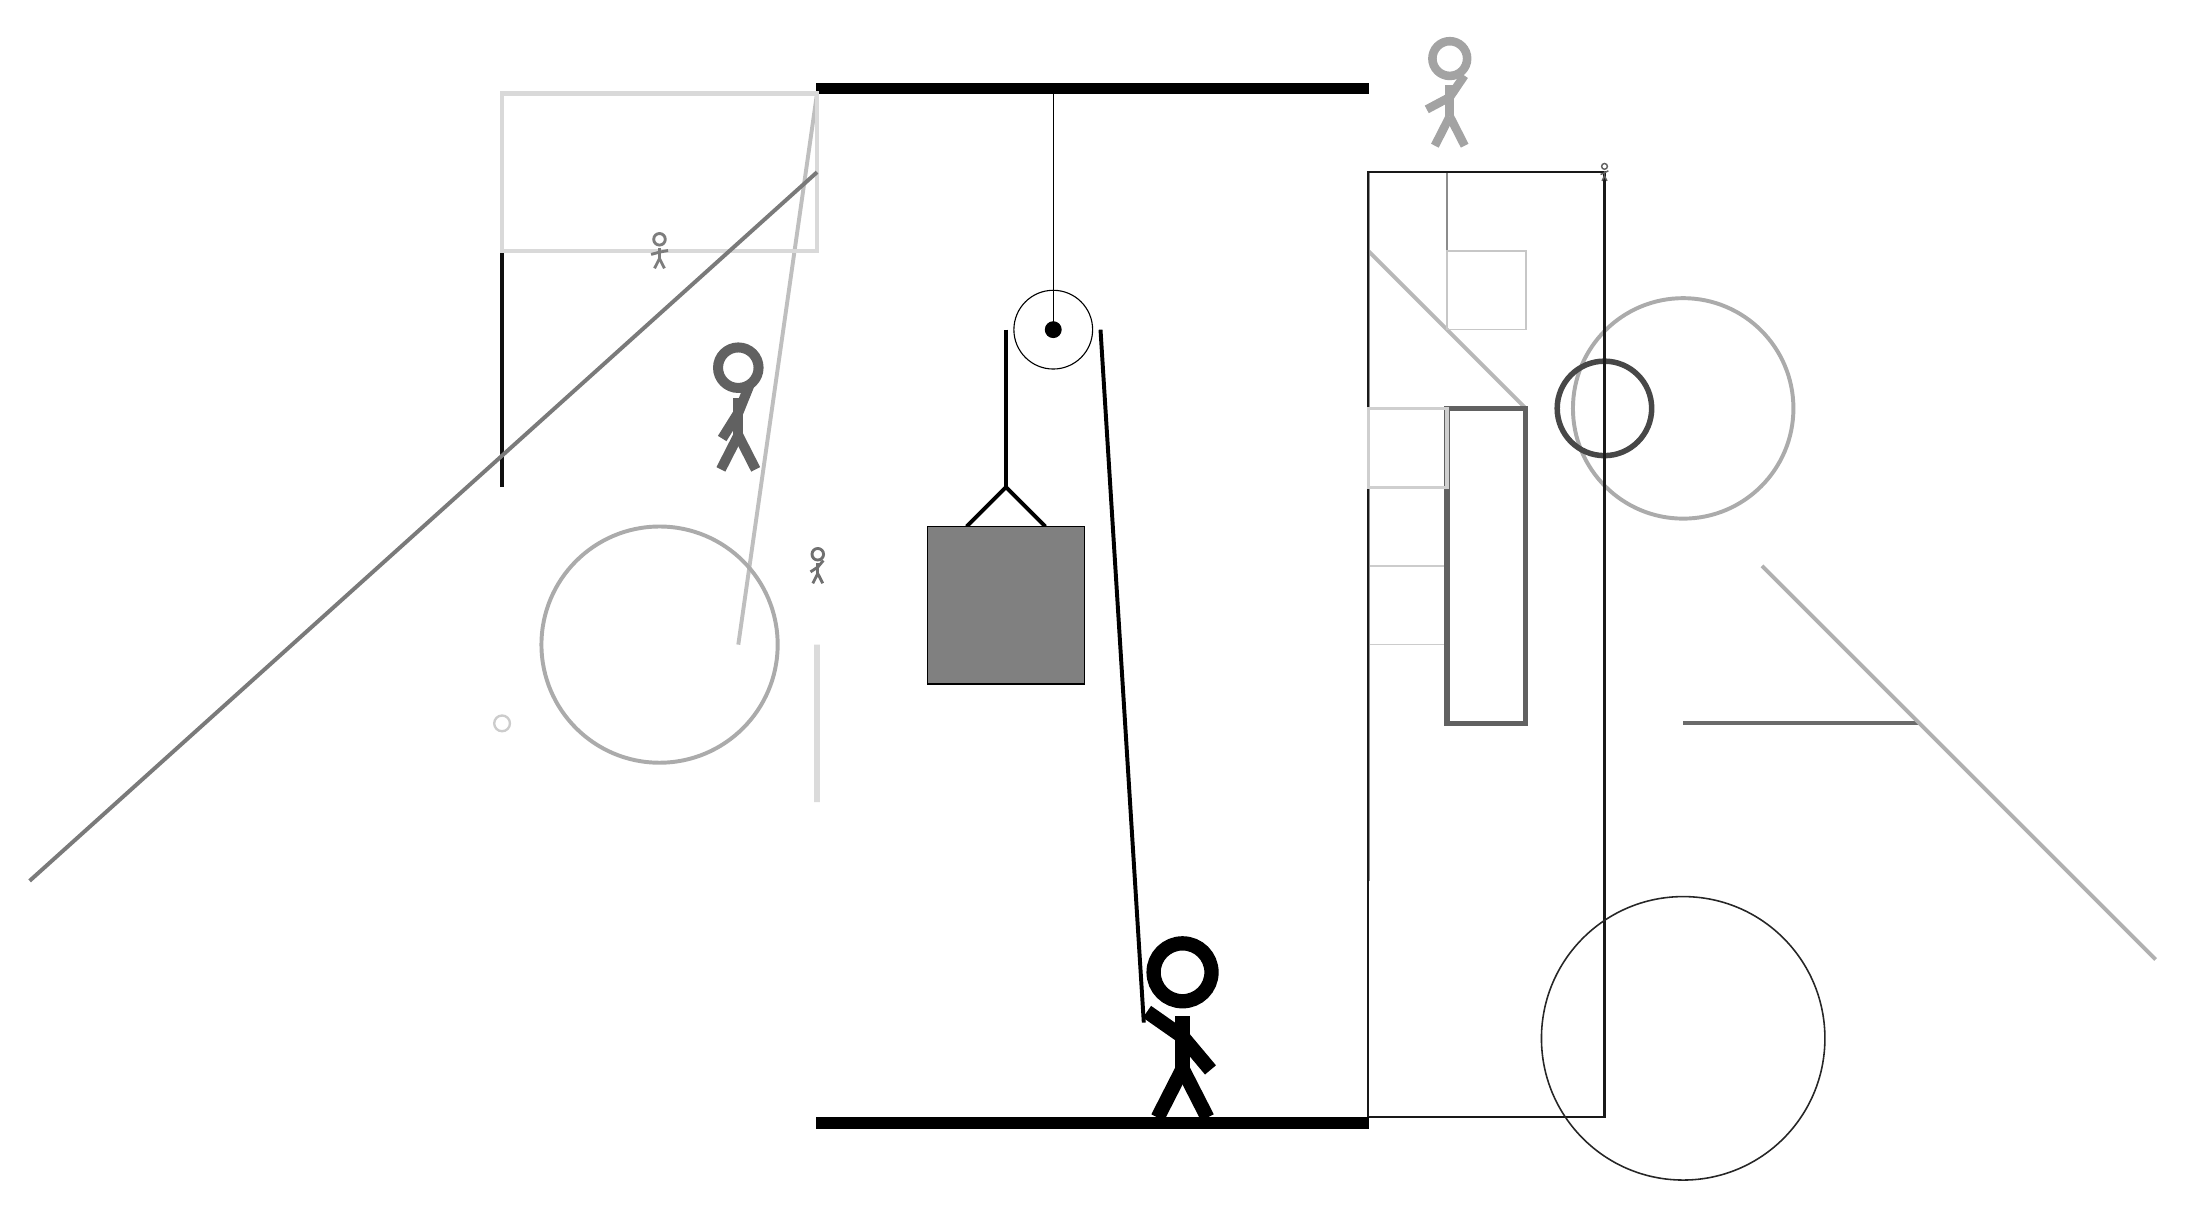
\begin{tikzpicture}
		%%%%% START %%%%%
		
		\draw[fill=black] (-2, 10) rectangle (5, 10.125);
		
		\draw (1, 7) circle (0.5);
		\draw[fill=black] (1, 7) circle (0.1);
		\draw (1, 10) -- (1, 7);
		
		\draw[line width=0.7mm, color=black!14] (-2, 1) rectangle (-2, 3);
		
		\draw[line width=0.5mm, color=black!58](9, 2) -- (12, 2);
		\draw[line width=0.5mm, color=black!25](-2, 10) -- (-3, 3);
		\draw [line width=0.3mm, color=black!20](-6, 2) circle (0.1);
		\draw[line width=0.5mm, color=black!94](-6, 5) -- (-6, 8);
		
		\draw [line width=0.5mm, color=black!33](9, 6) circle (1.4);
		
		\draw[line width=0.6mm, color=black!15] (-2, 10) rectangle (-6, 8);
		\draw[line width=0.5mm, color=black!28](7, 6) -- (5, 8);
		\draw[line width=0.2mm, color=black!20] (6, 3) rectangle (5, 4);
		
		\draw[line width=0.4mm, color=black!44] (5, 9) rectangle (5, 0);
		
		\node[line width=0.3mm, color=black!56] at (-2, 4) {\Strichmaxerl[2][33][50]};
		\draw[line width=0.2mm, color=black!45] (6, 7) rectangle (6, 9);
		\draw [line width=0.7mm, color=black!72](8, 6) circle (0.6);
		
		\draw[line width=0.3mm, color=black!90] (5, -3) rectangle (8, 9);
		\draw[line width=0.2mm, color=black!22] (7, 7) rectangle (6, 8);
		\draw[line width=0.5mm, color=black!52](-2, 9) -- (-12, 0);
		
		\node[line width=0.6mm, color=black!62] at (8, 9) {\Strichmaxerl[1][23][28]};
		\draw[line width=0.7mm, color=black!62] (6, 2) rectangle (7, 6);
		\node[line width=0.3mm, color=black!62] at (-3, 6) {\Strichmaxerl[7][58][68]};
		
		\draw [line width=0.5mm, color=black!33](-4, 3) circle (1.5);
		\node[line width=0.4mm, color=black!36] at (6, 10) {\Strichmaxerl[6][28][56]};
		\draw[line width=0.5mm, color=black!31](10, 4) -- (15, -1);
		\draw [line width=0.2mm, color=black!85](9, -2) circle (1.8);
		\node[line width=0.5mm, color=black!51] at (-4, 8) {\Strichmaxerl[2][15][11]};
		\draw[line width=0.4mm, color=black!19] (5, 6) rectangle (6, 5);
		
		
		\draw[line width=0.5mm] (-0.1, 4.5) -- (0.4, 5.0) -- (0.9, 4.5);
		\draw[fill=black!50] (-0.6, 4.5) rectangle (1.4, 2.5);
		
		\draw[line width=0.5mm] (0.4, 7) -- (0.4, 5.0);
		\centerarc[line width=0.5mm](1, 7)(0:180:0.6);
		\draw[line width=0.5mm](1.6, 7) -- (2.15, -1.8);
		
		\node at (2.6, -1.9) {\Strichmaxerl[10][-35][-50]};
		
		\draw[fill=black] (-2, -3) rectangle (5, -3.15);
		
		%%%%% END %%%%%
	\end{tikzpicture}
\end{document}